\begin{ZhChapter}

\chapter{實驗過程與結果}
\text 本章的版本比較為同一套RESTful API自動化測試系統逐步加入不同能力模組後之描述性結果，涵蓋規格理解、語意輸入建構、多代理測試實體化、工作流程決策與執行後恢復能力之累積演進。
\text 本章重點在於呈現系統能力演進與主要有效機制，而非演算法競賽式比較。v1至v2的評估以HTTP狀態碼為主要通過條件，其通過判定不包含操作間業務邏輯的語意合規性驗證；v3至v5則同步導入Manual Rule進行任務層級判定，兩組版本衡量的是不同層次的成功定義，通過率的絕對數值不宜直接比較。v4在v3基礎上加入工作流程決策分類模組，負責對執行結果進行狀態分類與事件記錄，作為離線策略訓練之資料來源；v5則以Offline-Q Policy為決策選擇器，於判定可恢復狀態時實際觸發恢復執行。差異僅在決策策略之選擇方式。因此，主要在變因控制上的比較，其結果可直接地反映兩種決策策略之有效情境差異。主要觀測指標為Workflow Recovered Pass，用以衡量工作流程恢復層於執行失敗後之實際恢復能力，此指標為v5 相對於v3、v4 之核心差異所在。

\section{開發環境與系統配置}
\text 本研究以Python作為主要開發語言，建置一套結合大型語言模型、多代理協作機制、工作流程引擎與離線強化學習決策策略之RESTful API自動化測試框架。整體系統採模組化架構設計，各功能模組透過工作流程狀態（Workflow State）進行資料交換，並由工作流程引擎統一管理執行順序。系統實作主要包含OpenAPI規格解析、多代理規格討論、測試案例生成、測試程式實體化、API執行、工作流程決策、離線策略訓練以及測試報告產生等模組。各模組皆以Python類別與函式實作，並透過LangGraph建立可追蹤之工作流程圖，以支援節點級執行紀錄與狀態管理。
\text 在大型語言模型整合方面，本研究採用可替換式模型介面設計，透過統一提供者層（Provider Layer）支援不同模型供應商。多代理協作部分則以AutoGen作為代理對話框架，負責規格討論、測試案例審查與測試程式生成等任務。工作流程控制則由LangGraph負責節點編排與狀態傳遞。此外，為支援工作流程決策策略之研究，本系統額外建置離線轉移資料集模組，用於記錄工作流程狀態、決策行動、獎勵值與下一狀態，並透過表格式擬合Q值迭代（Tabular Fitted Q Iteration）訓練離線工作流程決策策略。

表\ref{tab:implementation_environment}整理本研究主要開發環境與系統元件。

\begin{table}[H]
\centering
\caption{系統開發環境與主要元件}
\label{tab:implementation_environment}
\renewcommand{\arraystretch}{1.3}
\begin{tabular}{p{4cm} p{8cm}}
\toprule
\textbf{項目} & \textbf{內容} \\
\midrule
程式語言 & Python 3.14 \\
工作流程框架 & LangGraph \\
多代理框架 & AutoGen \\
大型語言模型介面 & OpenRouter / OpenAI Compatible API \\
API規格格式 & OpenAPI Specification 3.0.3 \\
測試執行方式 & HTTP Runtime Execution、Pytest Materialization \\
狀態管理 & Workflow State \\
決策策略 & Rule-based Policy、Offline-Q Policy \\
離線學習方法 & Tabular Fitted Q Iteration \\
資料格式 & JSON、JSONL、OpenAPI YAML \\
報告輸出 & JSON Report、Execution Trace、Policy Analysis Report \\
\bottomrule
\end{tabular}
\end{table}

\section{資料來源與測試目標}
\text 本研究之RESTful API測試環境主要採用RESTGPT研究所公開之測試資料作為基礎來源\parencite{Song2023RestGPT}。RESTGPT研究整理多個具備OpenAPI規格文件之公開RESTful API服務，並針對不同API建立對應之任務描述（Task Description）與執行路徑（Gold Path）作為大型語言模型與真實世界API操作互動之驗證環境。考量本研究聚焦於RESTful API測試流程、跨操作資源依賴以及工作流程決策策略之驗證，而非重新建構大型API資料集，因此選擇RESTGPT所提供之TMDB（The Movie Database）資料集作為主要實驗環境。TMDB資料集提供完整OpenAPI規格文件、公開開發者平台以及涵蓋多種API情境，資料集數量充足且涵蓋查詢、建立、修改與刪除等多種操作類型，同時存在跨操作資源依賴關係。RESTGPT已整理100筆Gold Path任務案例，可作為測試案例驗證基準，適合作為工作流程導向API測試之研究案例。
\text 相較於重新建構任務資料集，直接採用RESTGPT已驗證之Gold Path能降低人工標註成本，並提高不同研究之間的可比較性。因此，本研究以RESTGPT之TMDB資料集作為主要測試來源，並以其100筆Gold Path作為測試任務基準。在實際執行環境方面，由於TMDB API需要授權驗證，本研究則自行申請TMDB開發者帳號並取得API Access Token，以建立可執行之Live Execution環境。所有API測試皆透過實際HTTP請求與TMDB公開服務進行互動，而非使用模擬回應（Mock Response）或離線Replay環境，以確保測試流程符合服務提供者之使用規範。
\text 本研究將RESTGPT提供tmdb dataset之query與solution納為Gold Path作為MCP Context建構流程，使後續規格討論、多代理推理、測試案例生成與工作流程決策皆能建立於相同知識來源之上。

表\ref{tab:tmdb_dataset_source}整理本研究所使用之API資料來源。

\begin{table}[htbp]
\centering
\caption{研究使用之API資料來源}
\label{tab:tmdb_dataset_source}
\renewcommand{\arraystretch}{1.3}
\begin{tabular}{p{4cm} p{10cm}}
\toprule
\textbf{項目} & \textbf{內容} \\
\midrule
資料來源 & TMDB API \\
來源研究 & RESTGPT \parencite{Song2023RestGPT} \\
API類型 & Public RESTful API \\
規格格式 & OpenAPI Specification \\
認證方式 & Bearer Token Authentication \\
測試環境 & Live Production API \\
取得方式 & 開發者帳號申請與授權取得 \\
用途 & OpenAPI解析、測試案例生成與工作流程決策驗證 \\
\bottomrule
\end{tabular}
\end{table}

\text 本研究之主要測試單位並非TMDB OpenAPI規格中的全部API端點，而是RESTGPT已整理完成之100筆Gold Path任務案例，後續工作流程生成、測試執行與策略比較皆以任務案例（Task Case）為主要分析單位。
% 圖\ref{fig:implementation_overview}為本研究系統實作之整體架構。

% \begin{figure*}[H]
% \centering
% \includegraphics[width=0.9\textwidth]{figures/system_implementation_overview.png}
% \caption{系統實作整體架構圖}
% \label{fig:implementation_overview}
% \end{figure*}

\section{Benchmark 設計}
\text 傳統RESTful API測試評估指標（如端點覆蓋率、程式碼覆蓋率或突變測試分數）主要針對單一HTTP請求之功能正確性與測試充分性進行衡量，難以反映跨操作資源依賴、授權流程、工作流程決策介入以及任務層級完成性等因素之影響。本研究目標不在於測量API端點的覆蓋廣度，而在於評估系統能否在具有明確任務目標、操作依賴與可接受失敗條件的情境下，完成具語意意義之API測試任務並正確作出工作流程決策。因此，本研究選用任務導向測試基準（Task-Oriented Benchmark）作為主要評估框架，以Task Case為分析單位，並以Manual Rule作為最終判定依據，而非僅依賴HTTP狀態碼。
\text 本研究之實驗評估採用的Benchmark設計是任務導向測試基準（Task-Oriented Benchmark）。若僅以單一HTTP請求是否成功作為評估標準，將難以衡量跨操作依賴、授權流程以及工作流程決策策略對整體測試任務之影響。本研究之主要實驗基準採用RESTGPT所提供之TMDB Task Dataset與Gold Path資料，並結合人工規則文件（Manual Rules）形成100筆任務導向測試案例（Task-Oriented Test Cases）。
\text 每一筆測試案例均包含：Task Description、Gold Path Solution、對應Manual Rule、預期輸入參數、預期輸出結果、可接受失敗條件（Acceptable Failure Conditions）
\text 不同於一般API Benchmark以單一HTTP請求作為評估單位，本研究以完整任務（Task）作為分析單位。每一個Task可能包含多個API操作與跨步驟資源依賴，因此更能反映真實API測試情境。
\text 於實驗執行過程中，系統根據Task Description產生測試案例並執行實際HTTP請求，最終結果由Manual Rule進行判定，而非僅依賴HTTP Status Code。此設計可避免將語意錯誤之請求誤判為成功案例。

表\ref{tab:manual_doc_benchmark_definition}整理主實驗Benchmark之定義。

\begin{table}[H]
\centering
\caption{100-Case Manual Document Benchmark定義}
\label{tab:manual_doc_benchmark_definition}
\renewcommand{\arraystretch}{1.3}
\begin{tabular}{p{4cm} p{8cm}}
\toprule
\textbf{項目} & \textbf{內容} \\
\midrule
Benchmark名稱 & Manual Document Benchmark \\
資料來源 & RESTGPT TMDB Dataset \\
測試單位 & Task Case \\
案例數量 & 100 \\
評估方式 & Manual Rule Evaluation \\
執行環境 & Live Execution \\
主要用途 & v1～v5主實驗比較 \\
\bottomrule
\end{tabular}
\end{table}

\text 為評估不同技術元件對API測試流程之影響，本研究建立五個逐步演進版本（v1～v5），並於相同測試環境下執行比較。
\begin{table}[H]
\centering
\caption{v1～v5版本定義}
\label{tab:version_definition}
\renewcommand{\arraystretch}{1.3}
\begin{tabular}{p{1.5cm} p{10cm}}
\toprule
\textbf{Version} & \textbf{定義} \\
\midrule
v1 & Random / Monkey Execution Baseline \\
v2 & OpenAPI Specification + Seeded Input Generation \\
v3 & Manual Parsing + Multi-Agent Test Materialization \\
v4 & v3 + Rule-based Workflow Decision Policy \\
v5 & v3 + Offline-Q Workflow Decision Policy \\
\bottomrule
\end{tabular}
\end{table}

\paragraph{Version 1：Random Execution Baseline}
\text Version 1為最基礎之Baseline，使用 HTTP 層評估。系統僅根據OpenAPI端點資訊產生隨機測試請求，不使用Manual Rule、不建立語意輸入，也不進行跨步驟依賴推理。此版本主要用於觀察完全缺乏語意資訊時之基礎通過率。
\paragraph{Version 2：Specification-Guided Execution}
\text Version 2加入OpenAPI Specification解析與Seeded Input Generation。系統可利用規格資訊產生較合理之測試輸入，降低無效請求比例，但仍未導入多代理協作與工作流程決策機制。
\paragraph{Version 3：Multi-Agent Test Materialization}
\text Version 3於Version 2基礎上加入多代理協作機制後，同步導入 Manual Rule。系統透過Specification Discussion分析規格限制與依賴關係，並由Test Author與Test Reviewer共同產生可執行測試程式。此版本代表本研究完整測試生成能力，但尚未具備工作流程恢復能力。
\paragraph{Version 4：Rule-based Workflow Decision Policy}
\text Version 4於Version 3基礎上加入工作流程決策模組。系統根據HTTP Status Code、Semantic Error Type、Dependency Status以及Retry History等訊號，透過預先定義之規則對工作流程決策行動進行分類標記，並將狀態、行動、獎勵與後續狀態記錄為WorkflowDecisionEvent，作為後續Offline-Q策略訓練之離線轉移資料集。
\paragraph{Version 5：Offline-Q Workflow Decision Policy}
\text Version 5保留Version 3之所有測試生成能力，並以Offline-Q Policy取代Rule-based Policy作為學習型決策選擇器。系統首先利用既有Workflow Decision Events建立Offline RL Dataset，再透過Tabular Fitted Q Iteration訓練Workflow Decision Q-Policy。於執行期間，系統將WorkflowDecisionState轉換為State Feature Key，並查詢Q Table取得預期回報最高之恢復行動。Version 5之目的在於驗證工作流程決策是否可透過離線狀態--動作價值學習加以建模，並探索學習型策略在執行後恢復情境中的可行性與限制。

\subsection{Evaluation Metrics}

\text 為客觀評估不同版本之RESTful API自動化測試能力，本研究建立統一之任務導向（Task-Oriented）評估指標。所有版本均使用相同Task Dataset、相同Manual Rule、相同TMDB API環境以及相同身份驗證設定，以降低外部因素對比較結果之影響。本研究主要使用Task-Level Success作為評估基礎，並配合Workflow Recovery相關指標進行分析。
\text 由於本研究之測試單位為Task Case，而非單一HTTP請求，因此評估結果以任務層級（Task-Level）進行統計。每一個Task可能包含多個API操作、跨步驟資源依賴以及多次工作流程決策，因此單一HTTP狀態碼不足以作為最終判定依據。
\text 本研究主要採用Pass Rate、Strict Pass、Acceptable Failure Pass以及Workflow Recovered Pass作為評估指標。

\subsubsection{Pass Rate}
\text Pass Rate用於衡量整體任務成功比例，其定義如下：

\begin{equation}
PassRate=
\frac{N_{Pass}}
{N_{Total}}
\times100\%
\end{equation}

其中，$N_{Pass}$為成功完成之Task數量。
其中，$N_{Total}$為Benchmark總Task數量。Pass Rate為本研究主要比較指標，用於評估不同版本整體API測試能力之差異。

\subsubsection{Strict Pass}
\text Strict Pass代表測試案例完全符合Gold Path與Manual Rule所定義之預期結果。判定條件包含：HTTP回應成功、必要欄位存在、回應內容符合Manual Rule。Strict Pass代表系統成功完成預期測試目標，且不存在語意偏差。

\subsubsection{Acceptable Failure Pass}
\text 實際RESTful API測試環境中，部分API操作可能因權限限制、帳號限制或服務端策略而無法成功執行。若系統成功識別此類限制，並依據Manual Rule判定其屬於預期可接受失敗（Acceptable Failure），則該案例可被標記為Acceptable Failure Pass。例如：權限不足（403 Forbidden）、TMDB帳號限制操作、不允許匿名建立資源、非公開API功能。此指標可避免將環境限制誤判為測試失敗。

\subsubsection{Workflow Recovered Pass}
\text Workflow Recovered Pass用於衡量工作流程決策策略之恢復能力（Recovery Capability）。若初始測試執行失敗，但系統透過工作流程決策模組採取適當恢復行動後成功完成任務，則該案例將被標記為Workflow Recovered Pass。例如：Refresh Token後重新執行成功、Resolve Resource後重新執行成功、Regenerate Test Data後成功、Retry後成功。此指標主要用於評估Version 4與Version 5決策策略之效果。

其定義如下：
\begin{equation}
RecoveryRate=
\frac{N_{Recovered}}
{N_{StrictFail}}
\times100\%
\end{equation}

\section{實驗流程}

\text 本研究之實驗主要分為四個部分，包含基準資料準備、版本比較實驗、工作流程決策資料蒐集以及離線策略訓練與驗證。
% 整體流程如圖\ref{fig:experimental_procedure}所示。
\text 第一部分為測試資料準備（Dataset Preparation）。本研究採用RESTGPT所提供之TMDB資料集作為測試環境，包含OpenAPI規格文件、100筆Gold Path任務案例、Task Dataset以及對應之Manual Rule。所有測試案例皆透過TMDB官方API進行實際執行（Live Execution），並使用開發者帳號所取得之授權資訊完成身份驗證。
\text 第二部分為版本比較實驗（Version Benchmarking）。本研究依序執行v1至v5五種版本，並於相同測試案例集合下比較各版本之測試通過率與執行結果。Version v1至v3主要用於驗證規格解析、輸入生成與多代理測試生成機制之效果；Version v4則加入Rule-based Workflow Decision Policy；Version v5則進一步導入Offline-Q Workflow Decision Policy。
\text 第三部分為工作流程決策事件蒐集（Workflow Decision Event Collection）。於v4版本執行期間，系統將所有工作流程決策過程記錄為Workflow Decision Event，內容包含當前工作流程狀態（State）、採取之決策行動（Action）、後續狀態（Next State）以及對應獎勵值（Reward）。此資料將作為離線強化學習訓練資料集之來源。
\text 第四部分為離線策略訓練與驗證（Offline Policy Training and Evaluation）。系統根據蒐集之Workflow Decision Event建構Offline RL Dataset，並使用Tabular Fitted Q Iteration訓練Offline-Q Policy。完成訓練後，將策略載入v5工作流程決策模組進行推論，並於相同測試環境下重新執行Benchmark，以評估Offline-Q Policy於工作流程決策階段之表現。
\text 透過上述四個部分，本研究建立由基準測試、決策事件蒐集、離線策略訓練到策略驗證之完整實驗，使工作流程決策策略之訓練與評估皆建立於相同之測試環境與資料來源上。

\text 本研究所提出之多代理RESTful API自動化測試框架，目標在於建立一套可從API規格輸入開始，自動完成規格解析、語意推理、測試案例生成、測試程式實體化、實際API執行、工作流程決策以及測試報告產生之完整測試流程。
\text 與傳統以OpenAPI規格直接產生測試請求之方法不同，本研究將大型語言模型（Large Language Model, LLM）、多代理系統（Multi-Agent System, MAS）、模型上下文協定（Model Context Protocol, MCP）、代理人對代理人協定（Agent-to-Agent Protocol, A2A）以及工作流程決策策略整合於同一執行架構中，使系統能在測試過程中保留規格語意、人工文件知識以及執行歷史資訊，並根據實際執行結果選擇後續處理策略。整體系統架構採用工作流程導向（Workflow-Oriented）設計，所有模組均透過共享工作流程狀態（Workflow State）交換資料，並由工作流程引擎統一管理執行順序與狀態傳遞。

% 圖 \ref{fig:implementation_architecture} 為本研究實作之整體系統架構。

% \begin{figure*}[H]
% \centering
% \includegraphics[width=0.95\textwidth]{figures/implementation_architecture.png}
% \caption{本研究系統整體架構實作}
% \label{fig:implementation_architecture}
% \end{figure*}

\text 整體執行流程可分為六個主要階段：工作流程控制層（Workflow Control Layer）、規格解析與知識建構層（Specification Processing Layer）、多代理協作層（Multi-Agent Collaboration Layer）、測試生成與執行層（Test Generation and Execution Layer）、工作流程決策層（Workflow Decision Layer）、報告與可觀測性層（Reporting and Observability Layer）。其中，工作流程控制層負責協調各模組執行順序；規格解析層負責建立API語意知識；多代理協作層負責規格討論與測試內容審查；測試生成與執行層負責產生並執行測試案例；工作流程決策層負責分析執行結果並決定下一步行動；報告層則負責產生測試結果與策略分析報告。

\text 系統啟動後，首先由MCP Context Bootstrap模組載入OpenAPI規格、任務資料集（Task Dataset）、Gold Path、Manual Rule與相關文件內容，建立後續測試所需之上下文資訊。完成初始化後，OpenAPI Parser解析API規格內容，擷取端點（Endpoint）、請求參數、回應格式、身分驗證需求以及相關結構資訊。
\text 規格解析完成後，系統進入Specification Discussion階段。此階段透過AutoGen多代理協作機制，由不同角色代理共同分析OpenAPI規格與人工文件之間的差異，推導測試限制條件、參數依賴關係以及語意約束，並產生統一的規格解讀結果。
\text 接著進入Seeded Input Generation階段。系統根據規格解析結果、人工規則與既有語意種子資料建立候選輸入集合（Seeded Input Dataset），作為後續測試案例生成之基礎。此步驟可降低隨機輸入導致之無效請求比例，提升測試案例之語意合理性。
\text 在Test Case Generation階段中，系統根據候選輸入資料與規格限制條件產生抽象測試案例（Abstract Test Cases），並建立測試案例摘要與參數上下文資訊。之後由Test Code Materialization模組將抽象測試案例轉換為可執行之Python測試程式碼，並同步產生代理審查紀錄與協作追蹤資訊。
\text 完成測試程式產生後，API Execution模組負責執行實際HTTP請求，收集回應狀態碼、回應內容、執行時間與錯誤資訊。執行期間亦同步產生測試遙測資料（Telemetry）、執行軌跡（Execution Trace）與工作流程決策訊號（Workflow Decision Signal）。
\text 當測試執行完成後，系統進入Workflow Decision 階段。此階段將執行結果轉換為WorkflowDecisionState，並交由工作流程決策策略進行分析。根據目前研究版本不同，系統可選擇 Rule-based Workflow Policy 或 Offline-Q Workflow Policy 決定下一步行動，例如重新執行請求、重新產生測試資料、重新整理授權資訊、重新建立依賴資源，或直接產生報告。
\text 最後，Report Generation模組整合測試結果、執行紀錄、決策資訊與策略分析結果，輸出JSON格式測試報告、版本比較報告、策略分析報告以及工作流程決策紀錄，作為後續實驗分析與離線策略訓練之基礎資料來源。
\text 為支援跨模組資訊交換，本研究於系統內部統一採用Workflow State作為資料傳遞媒介。各節點不直接存取其他節點之內部資料，而是透過Workflow State中所維護之結構化欄位進行資訊交換。此設計可降低模組耦合度，並提升工作流程之可追蹤性、可維護性與可重播能力。
表\ref{tab:system_modules}整理本研究主要模組與其功能。

\begin{table}[H]
\centering
\caption{系統主要模組與功能}
\label{tab:system_modules}
\renewcommand{\arraystretch}{1.3}
\begin{tabularx}{\textwidth}{>{\raggedright\arraybackslash}p{4.4cm} >{\raggedright\arraybackslash}X}
\toprule
\textbf{模組} & \textbf{主要功能} \\
\midrule
\path{Workflow Engine} &
管理節點執行順序、狀態傳遞與控制 \\
\path{OpenAPI Processing} &
解析OpenAPI規格、建立端點資訊與欄位語意 \\
\path{MCP Context Builder} &
整合OpenAPI、Manual Document與Gold Path資訊 \\
\path{Multi-Agent Collaboration} &
執行規格討論、需求推理與測試內容審查 \\
\path{Seeded Input Generator} &
建立語意感知測試輸入資料 \\
\path{Test Case Generator} &
產生抽象測試案例與測試策略 \\
\path{Test Code Materializer} &
產生可執行測試程式 \\
\path{Runtime Executor} &
執行實際API請求與測試流程 \\
\path{Workflow Decision Module} &
分析執行結果並決定後續工作流程行動 \\
\path{Offline-Q Module} &
訓練與載入離線決策策略 \\
\path{Reward Evaluation Module} &
計算狀態轉移獎勵與PRM分數 \\
\path{Report Generator} &
產生測試報告與策略分析結果 \\
\bottomrule
\end{tabularx}
\end{table}

\text 此設計使所有節點皆能透過共享狀態存取前序節點產生之資訊，而不需直接耦合特定模組。整體執行實驗流程由LangGraph工作流程圖驅動，主要執行流程如下：
% 圖 \ref{fig:workflow_runtime_flow} 顯示系統於執行期間之資料流向。

% \begin{figure*}[H]
% \centering
% \includegraphics[width=0.95\textwidth]{figures/workflow_runtime_flow.png}
% \caption{系統執行期間之工作流程資料流}
% \label{fig:workflow_runtime_flow}
% \end{figure*}
\text 本研究架構並非單一線性流程，而是以Workflow State作為共同資料交換中心。OpenAPI處理模組、多代理協作模組、測試生成模組與執行模組皆透過共享狀態進行資訊交換。Decision Agent則負責接收執行結果並觸發工作流程決策策略，而Offline-Q模組與Reward模組則提供決策分析與策略推論能力。此種設計可降低模組間直接耦合程度，同時保留工作流程執行歷程，使後續測試分析、策略比較與執行回放皆能建立於相同資料結構之上。
\text 其中規格資訊流主要由OpenAPI 規格、Manual Rule與Manual Parse組成；執行資訊流則包含測試案例、測試程式碼、HTTP回應與執行紀錄；決策資訊流則包含WorkflowDecisionState、WorkflowDecisionSignal、Reward Breakdown以及Offline Reinforcement Learning Transition Record。透過三種資料流的整合，本系統能夠將 API 測試由單次請求驗證擴展為具備決策能力與恢復能力之工作流程測試架構。


\subsection{Offline-Q 工作流程決策策略設定}

\begin{table}[H]
\centering
\caption{Offline-Q工作流程決策策略設定}
\label{tab:offline_q_policy_config}
\scriptsize
\renewcommand{\arraystretch}{1.4}
\begin{tabularx}{\textwidth}{p{3.5cm} p{5.5cm} X} % 改用 tabularx，最後一欄自動延伸
\toprule
\textbf{項目} & \textbf{設定} & \textbf{說明} \\
\midrule
Policy Version & \texttt{offline\_q} & v5使用之離線Q值策略版本。 \\
Training Algorithm & \texttt{tabular\_fitted\_q\_iteration} & 以表格式擬合Q值迭代更新狀態-動作價值。 \\
Training Status & \texttt{trained\_tabular\_fitted\_q} & 表示策略已完成離線Q值訓練。 \\
Discount Factor & 0.9 & 控制未來獎勵對目前決策的影響程度。 \\
Iterations & 25 & Q值反覆更新次數。 \\
Action Space Size & 5 & 包含 \path{retry}、\path{resolve_resource}、\path{refresh_token}、\path{regenerate_data} 與 \path{report}。 \\
\bottomrule
\end{tabularx}
\end{table}



\section{Manual Document Benchmark主實驗結果}
\text 本研究於相同TMDB Task Dataset、相同Manual Rule、相同人工文件結構化檔案\texttt{semantic\_restbench\_tmdb\_motified.csv}以及相同Live Execution環境下，分別執行Version 1至Version 5之測試流程，以評估不同技術元件對RESTful API自動化測試能力之影響。本研究以100筆由manual document與gold path定義之測試案例作為主要實驗基準。此實驗不同於完整OpenAPI端點層級測試，其分母並非所有可解析API端點，而是具備明確任務目標、必要輸入、預期結果與可接受失敗條件之manual-doc-grounded test cases。每一個測試案例皆依據manual rule判定最終結果，並分為strict pass、workflow recovered pass與fail三種類型。
\text 表\ref{tab:version_benchmark_results}顯示v1至v5於100筆測試案例上的主要結果。v1採用隨機測試方式，僅通過25筆，顯示未考慮規格與語意資訊時，測試請求容易產生無效參數與錯誤路徑。v2導入OpenAPI規格與seeded input後，通過率提升至72\%，表示規格感知與語意輸入建構能有效改善請求品質。v3加入manual parsing、seeded input與multi-agent materialization後，通過率為69\%。相較於v2，v3雖未進一步提升通過率，但其任務層級判定較嚴格，顯示更完整的測試實體化與manual rule檢查會重新過濾部分僅於HTTP層面成功之案例。
\text 需特別說明的是，v2與v3之間的通過率差異，主因在於兩者評估通過的層次不同，而非多代理機制導致測試品質退步。v1與v2的通過判定以HTTP端點回應成功為主要依據：系統對100筆案例執行跨操作API呼叫，只要各步驟均取得成功的HTTP回應即視為通過，但此標準並未驗證操作間的業務邏輯與任務語意是否實際達成。因此，v2的0.72中可能包含「HTTP層面回應成功、但未正確完成操作間跨步驟資源綁定或未達成任務語意目標」的案例。v3同步導入Manual Rule與多代理測試實體化後，評估轉為任務層級語意合規性，要求測試結果符合人工文件所定義的操作間依賴關係與任務完成條件，過濾掉表面HTTP成功但任務語意不符的案例。因此，v3的0.69是本研究第一個能正確衡量「100筆任務的操作間業務邏輯是否實際達成」的通過率；v2的0.72與v3的0.69衡量的是不同層次的成功定義，兩者之間的差異應理解為評估精確度的校正結果而非系統能力的退步。
\text v4加入rule-based workflow decision 分類模組後，整體通過率維持69\%，此結果符合v4之設計預期，v4之功能在於對工作流程決策行動進行分類標記與事件蒐集，本身不觸發恢復執行，因此任務層級通過率與v3相同為合理結果。v5進一步導入offline-Q runtime decision selector後，通過率提升至79\%。值得注意的是，v5之Strict Pass Rate仍為0.69，與v3及v4相同；其Final Pass Rate提升至0.79，且新增之10筆通過皆來自Workflow Recovered Pass。此結果表示，v5的主要效益不在於提升前段測試生成能力，而在於於執行後根據工作流程狀態恢復原本會失敗之任務。

\text 本輪主實驗中，Acceptable Failure Pass未觀察到通過案例，因此後續結果分析將以Strict Pass、Final Pass與Workflow Recovered Pass作為主要指標。值得注意的是，本章之v1至v5結果應理解為系統逐步加入規格感知輸入、多代理測試實體化、工作流程決策與恢復能力後的能力演進。特別是v4與v5之差異，除了決策選擇器形式不同外，而v5涉及恢復行動能否於執行期被有效觸發，因此其結果解讀應以機制分析為主。

\begin{table}[H]
\centering
\caption{Version Benchmark Results}
\label{tab:version_benchmark_results}
\scriptsize
\renewcommand{\arraystretch}{1.3}
\begin{tabularx}{\textwidth}{
>{\centering\arraybackslash}p{0.9cm}
>{\centering\arraybackslash}p{0.9cm}
>{\centering\arraybackslash}p{0.9cm}
>{\centering\arraybackslash}p{1.4cm}
>{\centering\arraybackslash}p{1.8cm}
>{\centering\arraybackslash}p{1.6cm}
>{\centering\arraybackslash}p{2.1cm}
>{\centering\arraybackslash}X}
\toprule
\textbf{Version} &
\textbf{Passed} &
\textbf{Failed} &
\textbf{Pass Rate} &
\shortstack{Strict\\Pass Rate} &
\shortstack{Final\\Pass Rate} &
\shortstack{Acceptable\\Failure Pass} &
\shortstack{Workflow\\Recovered Pass} \\
\midrule
v1 & 25 & 75 & 0.25 & 0.25 & 0.25 & 0 & 0 \\
v2 & 72 & 28 & 0.72 & 0.72 & 0.72 & 0 & 0 \\
v3 & 69 & 31 & 0.69 & 0.69 & 0.69 & 0 & 0 \\
v4 & 69 & 31 & 0.69 & 0.69 & 0.69 & 0 & 0 \\
v5 & 79 & 21 & 0.79 & 0.69 & 0.79 & 0 & 10 \\
\bottomrule
\end{tabularx}
\end{table}

\text 為量化不同版本之效益差異，本研究定義版本間通過率差異如式 \eqref{eq:pass_rate_delta} 所示：
\begin{equation}
\label{eq:pass_rate_delta}
\Delta_{\mathrm{pass}}(v_i,v_j)=PassRate(v_i)-PassRate(v_j)
\end{equation}
\text 另為量化工作流程恢復對v5之貢獻，本研究定義恢復增益如式 \eqref{eq:recovery_gain_v5} 所示：
\begin{equation}
\label{eq:recovery_gain_v5}
RecoveryGain(v5)=FinalPassRate(v5)-StrictPassRate(v5)
\end{equation}
\text 依本輪結果可得：
\begin{equation}
\label{eq:recovery_gain_v5_value}
RecoveryGain(v5)=0.79-0.69=0.10
\end{equation}
\text 此結果表示，v5相較於v3與v4所增加之10\%通過率，應優先解讀為執行後工作流程恢復層在特定錯誤型態下發揮作用的結果；其中，學習型決策策略扮演的是在既有恢復行動集合中進行狀態導向選擇的角色，而非單獨產生全部增益來源。

\text 進一步而言，本輪觀察到之恢復效益具有明確錯誤型態集中性。所有Workflow Recovered Pass均來自404資源依賴缺失，表示目前最穩定被驗證之能力，是系統在資源識別碼失效或跨步驟綁定缺失情境下，仍可透過資源解析與第二次執行完成任務。對其他錯誤型態之恢復能力，則仍需更多資料與對照分析支持。其可形式化表示如下：
\begin{equation}
\label{eq:decision_variable_set_ch4}
\mathcal{X}_{\mathrm{decision}}=
\left\{
\begin{aligned}
&HTTPStatus,\; ErrorType,\; AuthRequired,\; DependencyStatus,\\
&ResourceAvailability,\; SemanticValidation,\; RetryCount,\; TokenState,\\
&NeedRegenerateData,\; NeedRegenerateCode
\end{aligned}
\right\}
\end{equation}

\text 公式\eqref{eq:decision_variable_set_ch4}中，各決策變數之意義如下：
\begin{itemize}
    \item $HTTPStatus$與$ErrorType$：用於辨識當前回應型態與錯誤來源。
    \item $AuthRequired$與$TokenState$：用於判斷是否屬於授權相關問題。
    \item $DependencyStatus$與$ResourceAvailability$：用於判斷是否存在可恢復之跨步驟資源缺失。
    \item $SemanticValidation$：用於識別是否屬於語意驗證錯誤。
    \item $RetryCount$：用於避免重複採取無效重試。
    \item $NeedRegenerateData$與$NeedRegenerateCode$：分別對應重新產生測試資料與重新產生測試程式之候選恢復方向。
\end{itemize}
\text 從主實驗結果觀察，工作流程決策的主要有效變數包含HTTP Status、Error Type、Dependency Status、Resource Availability與Retry Count。其中，HTTP Status與Error Type負責區分成功、驗證錯誤、授權錯誤、資源錯誤與環境錯誤；Dependency Status與Resource Availability則決定目前失敗是否可透過補足跨步驟資源而恢復；Retry Count則用於避免無效重試。相較之下，Token State與Semantic Validation雖仍屬正式決策變數，但在本輪100筆主實驗中，並非造成主要恢復增益之核心來源。
\text 為量化Benchmark Stability，本研究進一步定義基準執行穩定度如下：
\begin{equation}
\label{eq:benchmark_stability_ch4}
Stability=
\frac{N_{\mathrm{completed}}}
{N_{\mathrm{scheduled}}}
\end{equation}
\text 其中，$N_{\mathrm{completed}}$表示實際完成執行之任務數，$N_{\mathrm{scheduled}}$表示原定應執行之任務總數。於本輪主實驗中，$N_{\mathrm{completed}}=100$，$N_{\mathrm{scheduled}}=100$，故$Stability=1.0$；且\texttt{failed\_task\_runs=0}，表示至少在benchmark執行穩定性層面，本研究之實驗流程未因外部因素導致任務中止或批次失敗。
\text 從效益角度觀察，v1至v2之提升主要反映規格導向輸入建構對請求品質的改善；v2至v3則顯示Manual Rule的引入將評估層次從HTTP回應層提升至任務語意合規層，重新校正了任務層級通過率。v3至v4代表系統開始具備decision-aware baseline，但其Final Pass Rate仍未超出v3，顯示規則式決策層於本輪資料下尚未形成額外恢復增益。真正與本研究主題直接相關的效益發生於v5。雖然v5之Strict Pass Rate仍為0.69，與v3及v4相同，但其Final Pass Rate提升至0.79，表示decision layer並未改善前段生成品質，而是透過執行後之後續行動選擇改善workflow continuity。
\text 其次，就Workflow Recovery而言，v5新增10筆Workflow Recovered Pass，而v1至v4均為0，顯示離線決策策略已在部分情境下提供實質恢復能力。再次，就Oracle Match與Final Pass而言，v5之最終任務判定高於其Strict Pass，表示部分案例雖未於初始執行即成功，但能透過後續恢復步驟轉為最終成功。最後，就Benchmark Stability而言，本輪100筆任務均完成執行，且無失敗批次，表示此比較結果具備基本完整性。

\clearpage
\subsection{Workflow Recovery Analysis}
\text Version 5導入Offline-Q Workflow Decision Policy後，共有10筆案例於初始執行失敗後成功恢復，最終完成測試任務。表\ref{tab:workflow_recovery_cases}整理所有成功恢復案例。

\begin{table}[!htbp]
\centering
\caption{Workflow Recovery Cases in Version 5}
\label{tab:workflow_recovery_cases}
\scriptsize
\renewcommand{\arraystretch}{1.2}
\begin{tabularx}{\textwidth}{
>{\centering\arraybackslash}p{1.2cm}
>{\centering\arraybackslash}p{0.8cm}
>{\raggedright\arraybackslash}X
>{\raggedright\arraybackslash}p{2.2cm}
>{\centering\arraybackslash}p{0.9cm}
>{\centering\arraybackslash}p{0.9cm}
>{\raggedright\arraybackslash}p{1.9cm}
>{\centering\arraybackslash}p{1.3cm}}
\toprule
\textbf{Task ID} &
\textbf{Step} &
\textbf{Endpoint} &
\shortstack{\textbf{Recovery}\\\textbf{Action}} &
\textbf{Before} &
\textbf{After} &
\shortstack{\textbf{Resolved}\\\textbf{Binding}} &
\shortstack{\textbf{最終}\\\textbf{結果}} \\
\midrule
tmdb\_006 &
3 &
\path{/person/{person_id}/images} &
資源解析後重跑 &
404 &
200 &
\path{person_id=81247} &
恢復通過 \\

tmdb\_011 &
3 &
\path{/movie/{movie_id}/credits} &
資源解析後重跑 &
404 &
200 &
\path{movie_id=1236482} &
恢復通過 \\

tmdb\_020 &
3 &
\path{/movie/{movie_id}/images} &
資源解析後重跑 &
404 &
200 &
\path{movie_id=1236482} &
恢復通過 \\

tmdb\_023 &
3 &
\path{/movie/{movie_id}/release_dates} &
資源解析後重跑 &
404 &
200 &
\path{movie_id=1236482} &
恢復通過 \\

tmdb\_025 &
3 &
\path{/movie/{movie_id}/similar} &
資源解析後重跑 &
404 &
200 &
\path{movie_id=1236482} &
恢復通過 \\

tmdb\_044 &
3 &
\path{/person/{person_id}/movie_credits} &
資源解析後重跑 &
404 &
200 &
\path{person_id=81247} &
恢復通過 \\

tmdb\_085 &
3 &
\path{/person/{person_id}} &
資源解析後重跑 &
404 &
200 &
\path{person_id=81247} &
恢復通過 \\

tmdb\_086 &
3 &
\path{/person/{person_id}} &
資源解析後重跑 &
404 &
200 &
\path{person_id=81247} &
恢復通過 \\

tmdb\_087 &
3 &
\path{/company/{company_id}} &
資源解析後重跑 &
404 &
200 &
\path{company_id=81247} &
恢復通過 \\

tmdb\_091 &
3 &
\path{/person/{person_id}} &
資源解析後重跑 &
404 &
200 &
\path{person_id=81247} &
恢復通過 \\
\bottomrule
\end{tabularx}
\end{table}

\text 為量化v5之恢復效益，本研究定義恢復增益如式 \eqref{eq:recovery_gain_v5_subsection} 所示：
\begin{equation}
\label{eq:recovery_gain_v5_subsection}
RecoveryGain(v5)=FinalPassRate(v5)-StrictPassRate(v5)
\end{equation}
\begin{equation}
\label{eq:recovery_gain_v5_subsection_value}
RecoveryGain(v5)=0.79-0.69=0.10
\end{equation}

\text 另定義恢復率如式 \eqref{eq:recovery_rate_v5} 所示：
\begin{equation}
\label{eq:recovery_rate_v5}
RecoveryRate(v5)=
\frac{N_{Recovered}}
{N_{StrictFail}}
\end{equation}
\text 其中，$N_{Recovered}=10$，$N_{StrictFail}=31$，故可得：
\begin{equation}
\label{eq:recovery_rate_v5_value}
RecoveryRate(v5)=\frac{10}{31}\approx0.3226
\end{equation}

\text 分析結果顯示，所有成功恢復案例皆屬於資源識別碼失效所導致之404 Not Found錯誤。當Offline-Q Policy判斷當前狀態符合資源缺失特徵時，系統會選擇\texttt{resolve\_resource\_and\_rerun}作為恢復行動，並透過Resource Pool重新取得有效資源識別碼後再次執行測試。
\text 此結果表示，本輪主實驗中最具辨識力之決策變數組合為HTTP Status、Error Type、Dependency Status與Resource Availability。換言之，v5目前最主要學到的是「404 + 資源依賴缺失」情境下之工作流程恢復模式，而非全面性涵蓋所有錯誤類型之恢復策略。
\text 進一步觀察表~\ref{tab:workflow_recovery_cases}之資源識別碼分布可知，10筆恢復案例中，\path{person_id=81247}出現於tmdb\_006、tmdb\_044、tmdb\_085、tmdb\_086、tmdb\_091共5筆案例，\path{movie_id=1236482}出現於tmdb\_011、tmdb\_020、tmdb\_023、tmdb\_025共4筆案例，底層資源綁定失效根因實際集中於約2至3類不同的跨步驟資源缺失情境。此觀察顯示，RecoveryRate所反映的，是系統在特定資源識別碼缺失型態下具備穩定的持續執行能力——相同根因在多個任務案例中均能被成功恢復，本身即為恢復層穩定性的正面佐證——而非10種完全獨立的異質恢復情境均已得到驗證。因此，對當前恢復能力較準確的定位應為：系統已在「跨步驟資源識別碼缺失」此一特定情境下展現穩定的後執行恢復能力；對其他錯誤型態下的恢復廣度，仍需更多樣化的執行資料加以補充。

\subsection{v4與v5之差異分析}
\text v4與v5之比較設計，其核心定位在於對照兩種典型的工作流程決策情境。v4代表目前主流結合大型語言模型之API自動化測試工具的典型能力邊界：系統能夠解析規格、生成測試案例並執行測試，於遭遇失敗時對工作流程決策行動進行分類標記與事件記錄，但本身不觸發實際恢復行動。此模式對應於現行多數LLM輔助測試框架的實際運作方式——能夠理解規格語意，但在執行障礙後選擇停止，而非嘗試恢復。v5則為本研究Offline-Q策略學習之實驗設計，透過離線強化學習所訓練之Q-Policy，於執行失敗後根據工作流程狀態實際觸發對應恢復行動，驗證學習型工作流程決策策略在執行後恢復情境中的可行性。因此，v4與v5之比較，其本質問題為：結合大型語言模型的API自動化測試，能否透過後執行工作流程決策策略，突破失敗即停止的能力邊界。

\text 因此，v4與v5之差異不宜簡化為rule-based與離線強化學習之純策略比較。較精確地說，v4主要代表decision-aware verdict baseline；v5則是在工作流程恢復機制存在時，進一步以學習型決策選擇器決定是否觸發資源解析、更新授權、重新產生資料或直接報告。故本研究目前最直接成立之結論，是工作流程恢復層與狀態導向決策可共同提升流程延續性，而非單獨宣稱Offline-Q已全面優於規則式策略。
\text 雖然v4與v5於本研究主實驗中之研究定位皆屬工作流程決策層版本，但兩者所代表的研究意義不同。v4主要驗證rule-based workflow decision 能否根據manual rule與錯誤分類，判斷非2XX結果是否仍屬於任務可接受結果。換言之，v4的功能重點在於workflow-level verdict，而非將失敗請求重新執行為成功結果。
\text 相較之下，v5導入offline-Q runtime decision selector，其目標是根據離線轉移資料集所學得之狀態--行動價值，於執行時選擇較合適的工作流程行動。就本輪主實驗結果而言，v4之Final Pass Rate為0.69，v5則提升至0.79；然而，v5之Strict Pass Rate仍為0.69，與v4相同。此結果表示，v5之額外提升並非來自前段測試生成品質改善，而是來自執行後工作流程恢復能力。
\text 更具體地說，v4使系統可在語意層級上避免將環境限制或資源缺失直接視為任務失敗；v5則進一步在部分404資源缺失情境中，透過資源池、manual binding pool與runtime value pool執行second-pass rerun，使原先失敗之請求重新取得成功結果，並轉為workflow recovered pass。
\text 綜合而言，本研究目前最直接成立之結論為：工作流程恢復層與狀態導向決策可共同提升流程延續性。此差異對RESTful API測試具有實務意義——在具操作間依賴之API任務中，系統從失敗狀態恢復並繼續執行後續步驟，其測試訊號價值高於單純將失敗結果標記為可接受。

\clearpage
\subsection{Offline-Q策略學習之深度診斷}
\text 本節說明 Offline-Q 策略學習之訓練結果、Q-table結構診斷，以及策略學習之有效邊界與限制。完成Offline Dataset建構後，本研究採用Tabular Fitted Q Iteration進行離線策略訓練，折扣因子（Discount Factor）設定為$\gamma=0.9$，共進行25次迭代更新。訓練結果如表~\ref{tab:q_training_summary}所示，最終Q-table包含60個states與62組state-action pairs。

\begin{table}[H]
\centering
\caption{Offline-Q訓練結果摘要}
\label{tab:q_training_summary}
\renewcommand{\arraystretch}{1.3}
\begin{tabular}{lc}
\toprule
\textbf{項目} & \textbf{數值} \\
\midrule
Policy Version & \texttt{v5\_offline\_q\_contrastive} \\
Training Algorithm & \texttt{tabular\_fitted\_q\_iteration} \\
Discount Factor ($\gamma$) & 0.9 \\
Training Iterations & 25 \\
Train Record Count & 139 \\
Validation Record Count & 29 \\
Train State Count & 60 \\
Validation State Count & 18 \\
Final Q-table States & 60 \\
Final State-Action Pairs & 62 \\
\bottomrule
\end{tabular}
\end{table}

\text 進一步觀察資料分布可知，目前訓練資料具有明顯之action不平衡。訓練集之行動分布如下：
\begin{itemize}
    \item \path{report=113}
    \item \path{resolve_resource=21}
    \item \path{regenerate_data=3}
    \item \path{refresh_token=1}
    \item \path{retry=1}
\end{itemize}
\text 訓練集大多來自「成功後進入報告」之記錄，低頻恢復型行動之覆蓋相對有限。

\paragraph{Q-table 結構診斷}
\text 對完整Q-table（圖\ref{fig:q_table}）進行結構性分析後，發現60個訓練狀態中，58個狀態僅含單一動作之Q值記錄，其餘行動欄位均為空值，代表這些狀態在訓練資料中從未觀察到其他行動被執行。在單一動作狀態下，$\max_{a'} Q(s', a')$退化為確定性常數，Fitted-Q迭代無法引入跨行動之相對價值比較。僅有2個狀態具備多動作對比記錄，可作為策略評估之對比狀態（contrastive states）。
\text 其中，S059（VALIDATION / status\_400 / auth\_bootstrap）中 \texttt{regenerate\_data} 之Q值為0.60、\texttt{report}為0.10，策略正確偏好恢復型行動；S060（VALIDATION / status\_400 / rating\_write）中 \texttt{report} 之Q值為0.55、\texttt{retry}為$-0.05$，為整個Q-table唯一出現負值之state-action pair，顯示策略已學得「對相同失敗狀態直接重試通常無效」之局部判斷。
\text 此結構直接解釋了 $\Delta Q^{(k)}$ 在全25次迭代均為0.0的現象（式~\eqref{eq:max_abs_q_delta}）：策略在第一次迭代後即收斂至由empirical reward與logged transition決定之固定點，現階段主要瓶頸並非迭代次數不足，而是dataset coverage。
\begin{equation}
\label{eq:max_abs_q_delta}
\Delta Q^{(k)}=
\max_{s,a}
\left|
Q^{(k)}(s,a)-Q^{(k-1)}(s,a)
\right|
\end{equation}
\clearpage
\begin{figure}[!htbp]
    \centering
    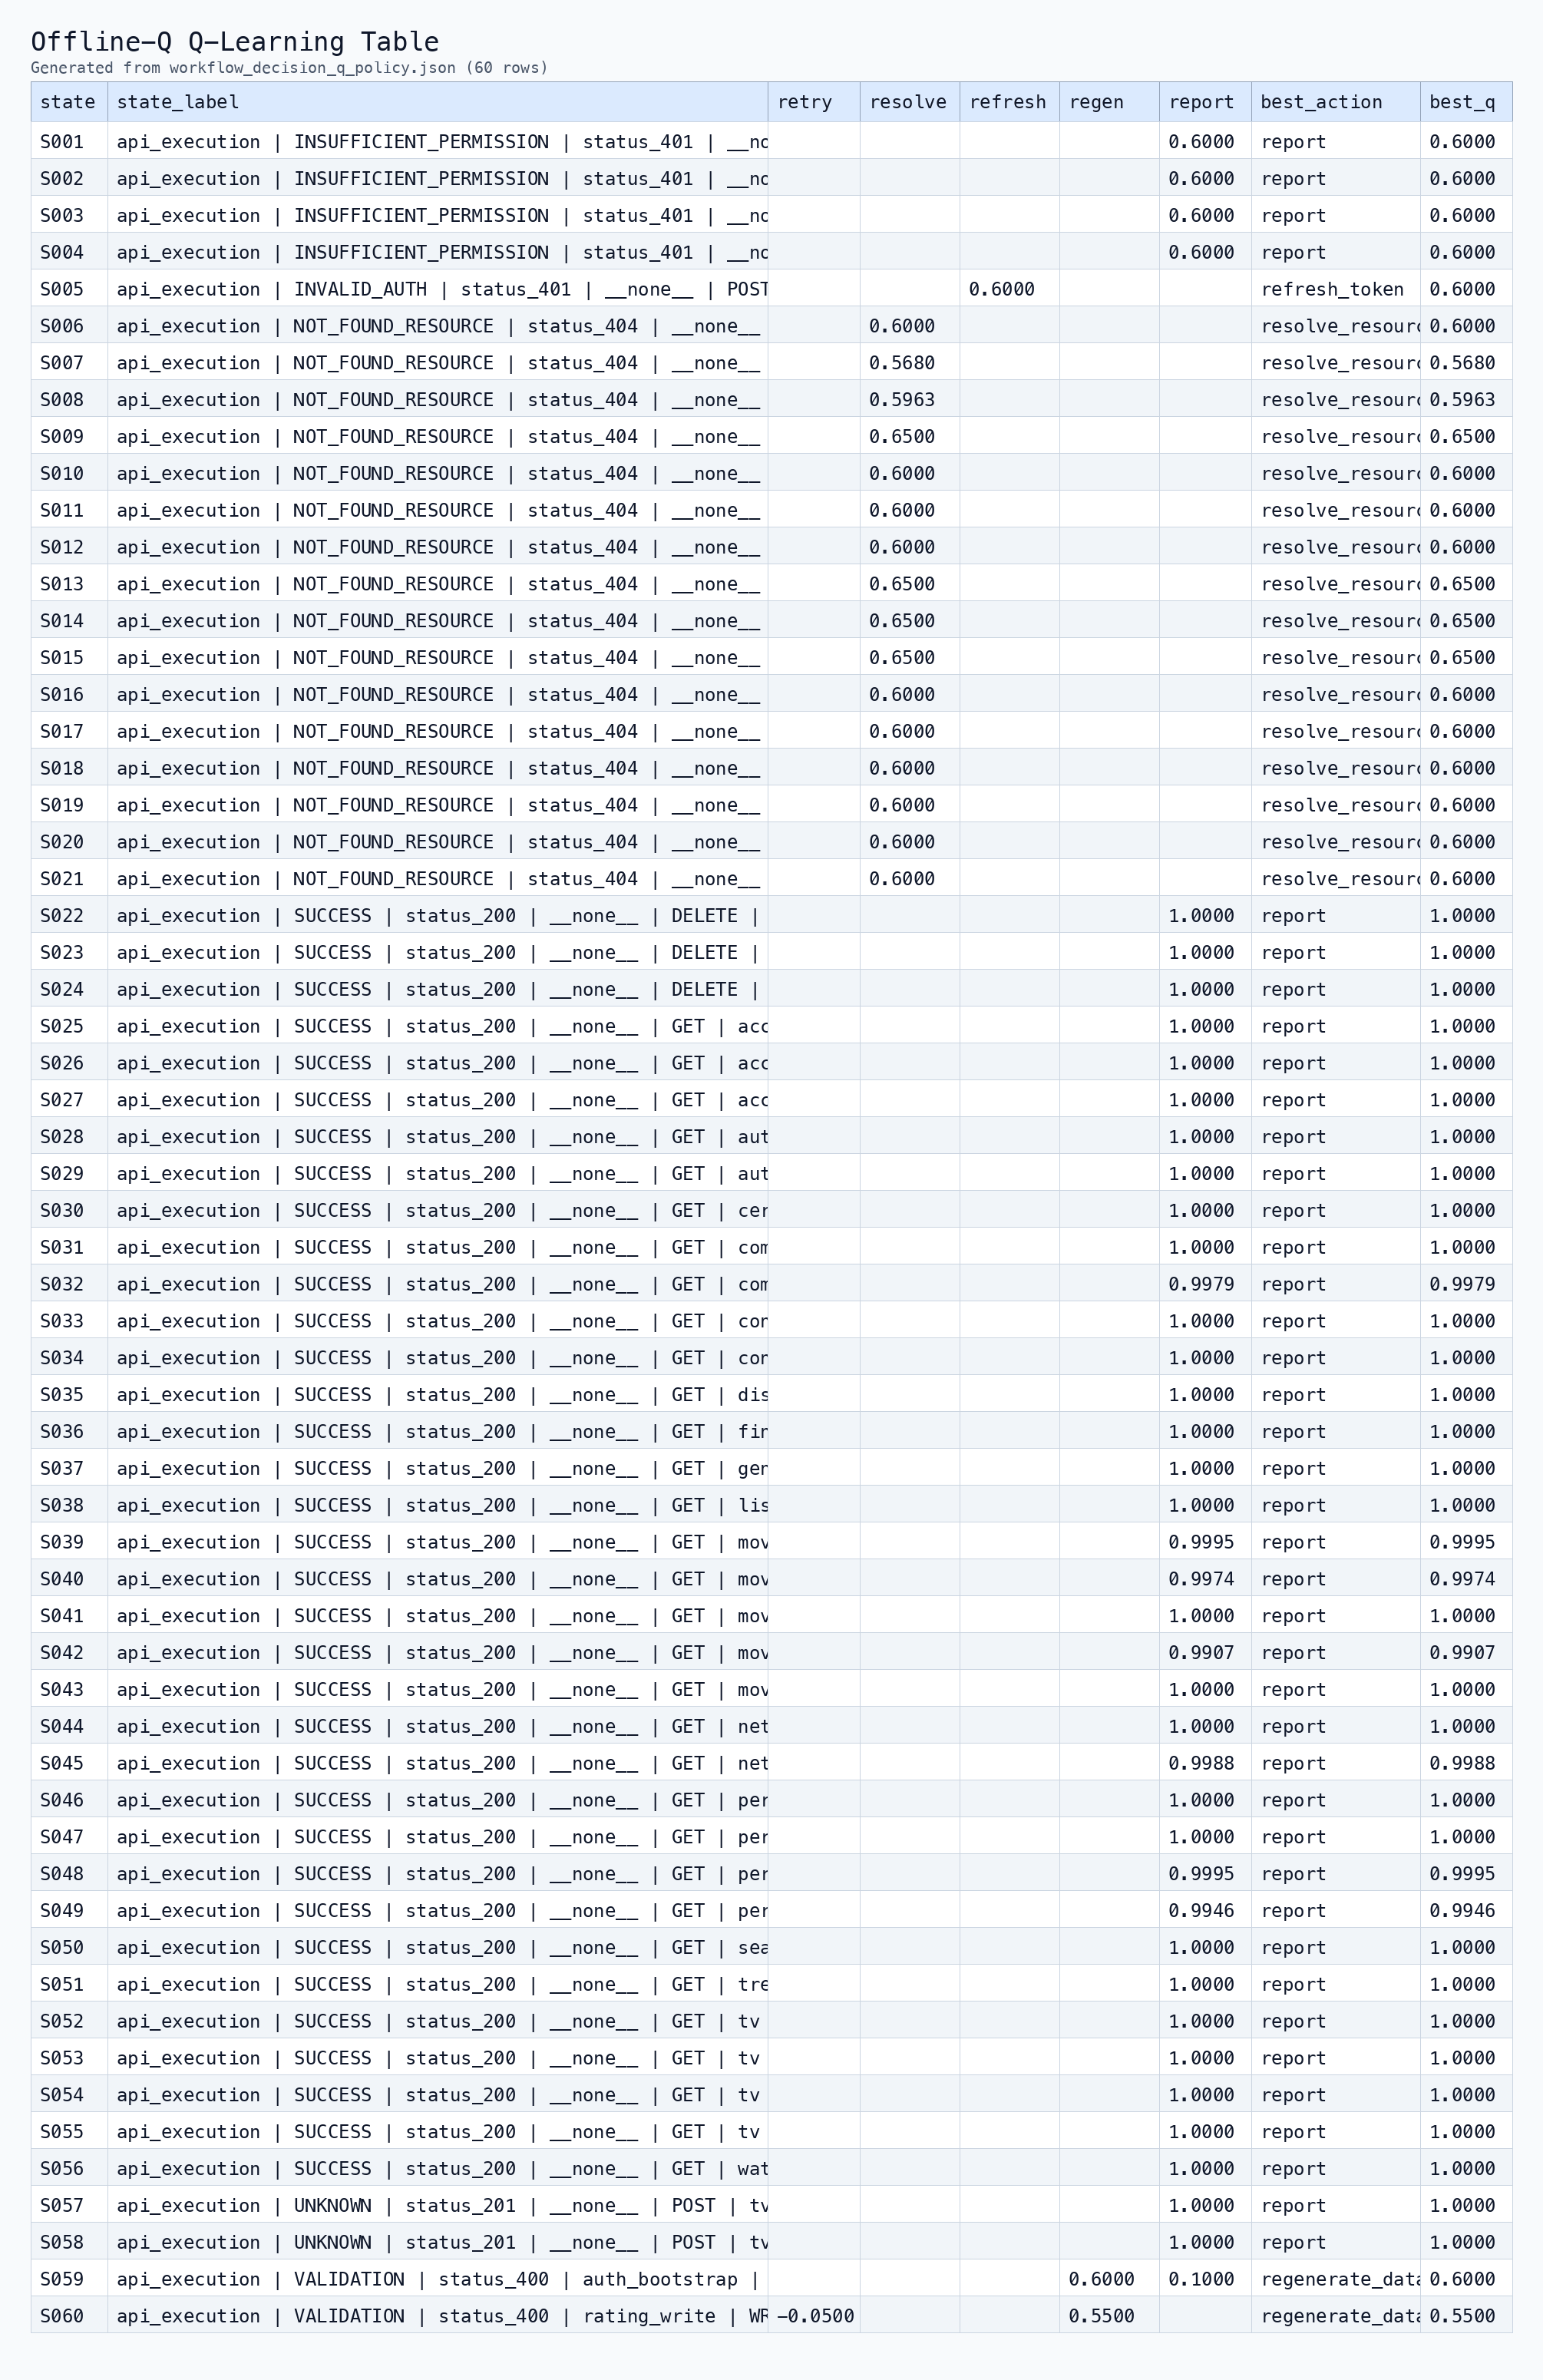
\includegraphics[width = 0.92\textwidth]{static-page/offline_q_learning_table.png}
    \caption{Offline-Q Policy之Q-table}
    \label{fig:q_table}
\end{figure}

\paragraph{Q-value 分布與行動偏好}
\text 在Q-value整體分布方面，本輪62個state-action pairs之統計結果為：最小值$-0.05$、最大值$1.00$、平均值$0.8217$、中位數$0.9995$，其中正值61筆、負值1筆。Q-value高度集中於1.0附近，顯示多數狀態下策略已穩定偏好「完成當前流程並進入報告」之行動。

\begin{figure}[!htbp]
    \centering
    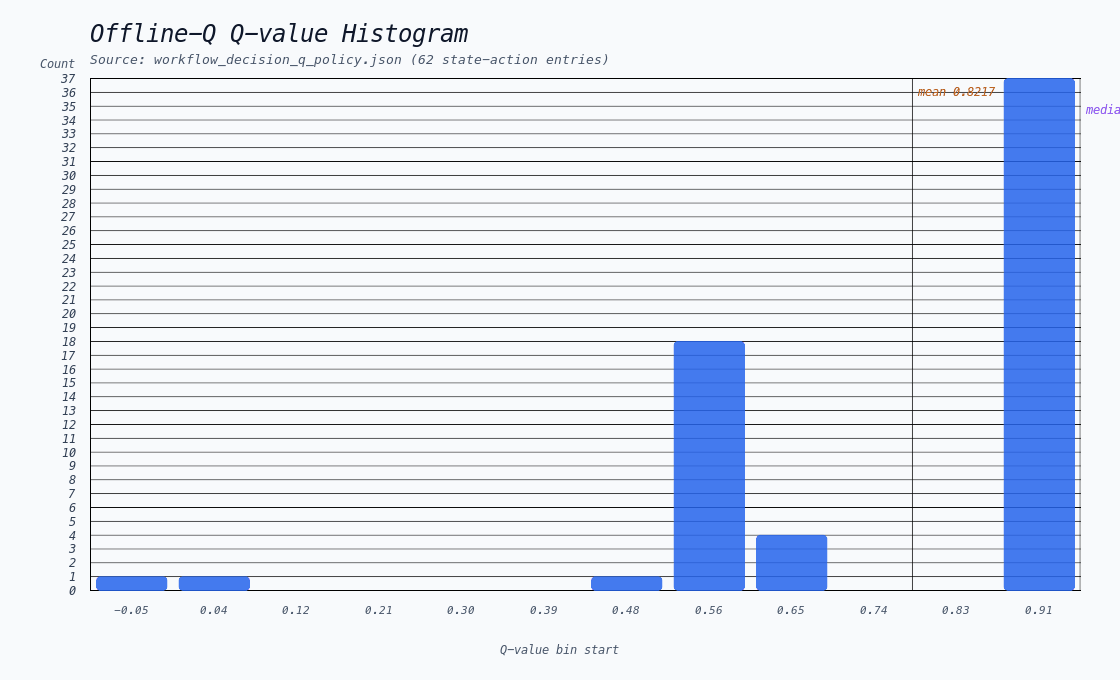
\includegraphics[width = 1.0\textwidth]{static-page/offline_q_value_histogram.png}
    \caption{Offline-Q Policy之Q-value分布}
    \label{fig:q_value_histogram}
\end{figure}

\begin{table}[!htbp]
\centering
\caption{Offline-Q各決策行動Q-value統計}
\label{tab:q_action_distribution}
\begin{tabular}{lccccc}
\toprule
Action &
Count &
Mean Q &
Max Q &
Positive &
Negative \\
\midrule
retry & 1 & -0.05 & -0.05 & 0 & 1 \\
resolve\_resource & 16 & 0.6103 & 0.65 & 16 & 0 \\
refresh\_token & 1 & 0.60 & 0.60 & 1 & 0 \\
regenerate\_data & 2 & 0.5750 & 0.60 & 2 & 0 \\
report & 42 & 0.9400 & 1.00 & 42 & 0 \\
\bottomrule
\end{tabular}
\end{table}

\text 表\ref{tab:q_action_distribution}顯示，不同行動之Q-value分布具有明顯差異。\texttt{report}擁有最高平均值與最大值，反映策略已穩定學到「於成功或已可明確歸因之狀態下結束流程」的偏好。於真正恢復型行動中，\texttt{resolve\_resource}之平均Q-value最高，\texttt{regenerate\_data}次之，而\texttt{retry}為唯一負值，表示在目前資料下，對相同失敗狀態直接重送相同請求通常無法帶來正向回報。


\begin{figure}[!htbp]
    \centering
    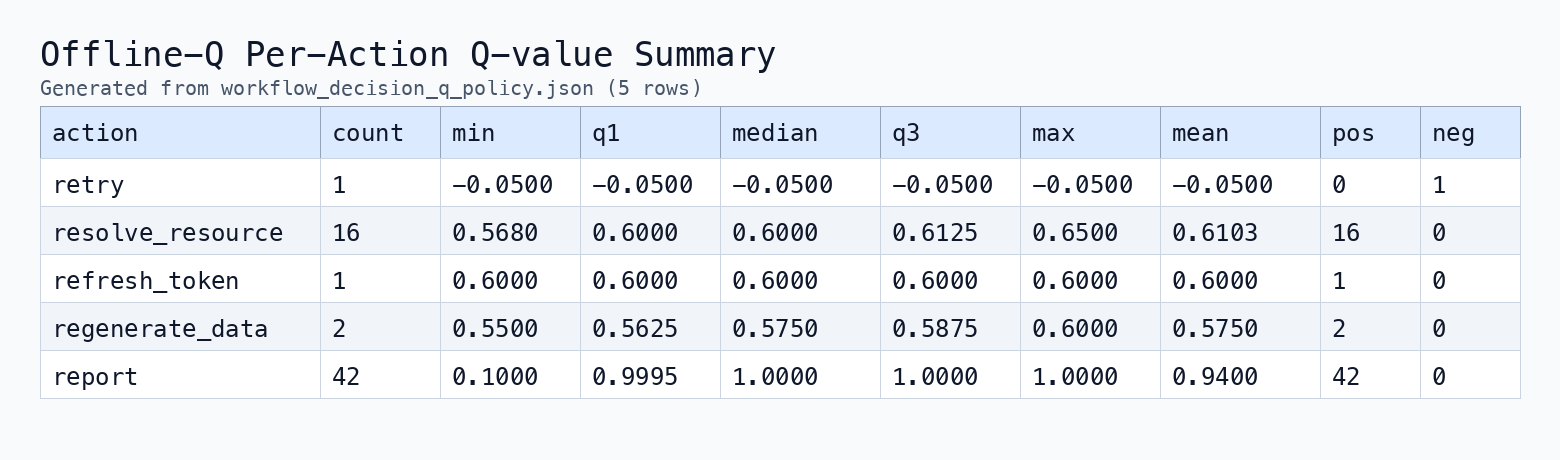
\includegraphics[width = 0.98\textwidth]{static-page/offline_q_per_action_summary_table.png}
    \caption{Offline-Q各決策行動之完整Q-value統計摘要}
    \label{fig:q_action_summary_table}
\end{figure}

\text 若將圖\ref{fig:q_action_summary_table}與圖\ref{fig:q_value_boxplot}併同觀察，前者提供各行動之分位數摘要，後者則提供分布形狀與離散程度之視覺化證據。兩者共同顯示，目前Offline-Q所學得之主要有效模式，集中於「成功後報告」與「404資源依賴缺失下進行資源解析」兩類狀態。
\text 為補充表\ref{tab:q_action_distribution}所呈現之平均值與正負值分布，圖\ref{fig:q_action_summary_table}進一步列出各決策行動之最小值、第一四分位數、中位數、第三四分位數、最大值與平均值。由圖可觀察到，\texttt{report}之第一四分位數已達0.9995，顯示多數成功後報告狀態之Q-value高度集中於1.0附近；\texttt{resolve\_resource}則集中於約0.60至0.65之區間，反映其為目前最穩定的恢復型行動；\texttt{retry}則仍為唯一負值行動，進一步支持其在現有資料覆蓋下並非有效策略。

\begin{figure}[!htbp]
    \centering
    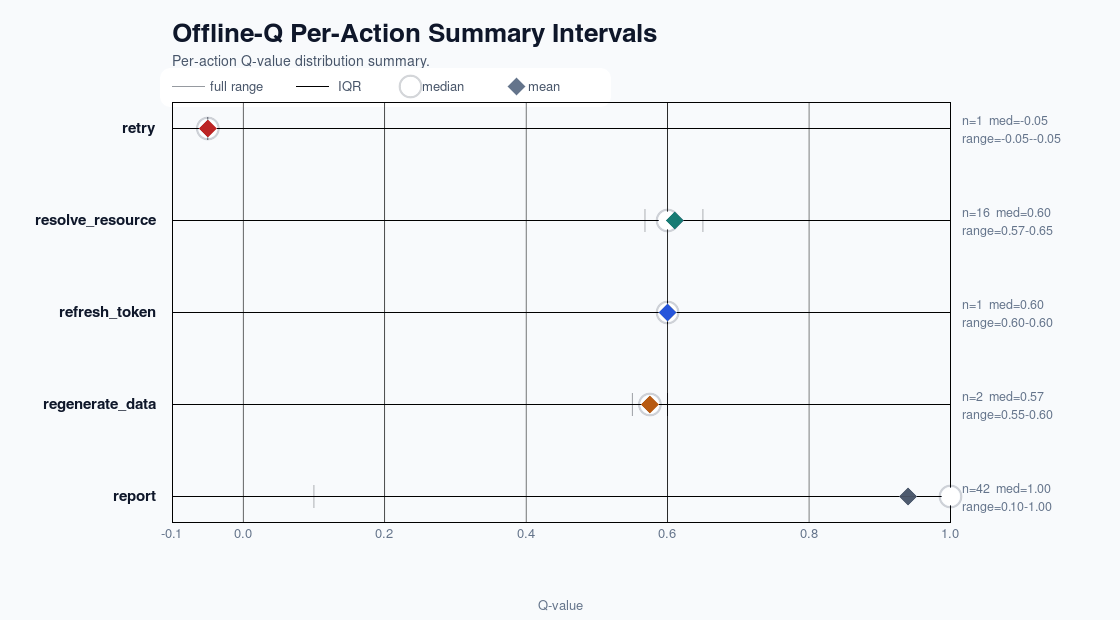
\includegraphics[width = 1.0\textwidth]{static-page/offline_q_value_lineplot_by_action.png}
    \caption{不同決策行動之Q-value分布}
    \label{fig:q_value_boxplot}
\end{figure}

\text 圖\ref{fig:q_value_boxplot}進一步依決策行動分析Q-value分布。結果顯示，\texttt{resolve\_resource}具有最高的恢復型Q-value分布，且與主實驗中10筆Workflow Recovered Pass皆來自404資源依賴缺失情境之觀察一致。這表示目前Offline-Q所學得的主要有效模式，集中於「404 Not Found + Dependency Missing」狀態下優先選擇資源解析與重新執行。

\text 另從最佳action分布觀察，每個state之最佳action分布為：\path{report=42}、\path{resolve_resource=16}、\path{refresh_token=1}與\path{regenerate_data=2}。此結果再次顯示，目前policy已明確區分兩類主要情境：其一為成功或已完成狀態，最佳行動為\texttt{report}；其二為可恢復之資源依賴錯誤狀態，最佳行動為\texttt{resolve\_resource}。

\paragraph{離線策略評估指標}
\text 為評估離線策略與logged behavior之相容程度，本研究採用matched action rate（式~\eqref{eq:matched_action_rate}）作為輔助指標。 訓練集MAR為 $137/139 = 0.9856$，驗證集為 $24/29 = 0.8276$；train direct-method policy value為0.9003，validation為0.8149。
\text 此結果顯示策略與既有行為高度一致，驗證集覆蓋落差則反映低頻行動在驗證資料中的分布更為稀疏。在當前資料規模與行動分布偏斜條件下，上述數值較適合用於說明策略與logged behavior之相容程度，而不宜單獨視為策略效能之強力證據。
\begin{equation}
\label{eq:matched_action_rate}
MAR=
\frac{N_{\mathrm{matched}}}
{N_{\mathrm{records}}}
\end{equation}

\paragraph{測試成本與資料蒐集偏誤之結構性分析}
\text 當前Q-table\ref{fig:q_table}呈現58/60狀態為單一動作記錄之結構，其根本成因是Live API測試環境中探索成本高昂所引發的資料蒐集偏誤（data collection bias）。
\text 在真實 API 測試情境中，主動探索低頻恢復行動（如對同一請求反覆嘗試 \texttt{retry} 或 \texttt{regenerate\_data}）會引發一系列現實代價：測試資料庫狀態污染、額外的網路延遲與API rate有限觸發，以及潛在的服務端異常風險。這些成本迫使資料蒐集過程採取保守的行為策略，僅記錄系統判斷為安全的行動，導致動作支撐集（action support）在多數狀態下退化為單一選項。
\text 從統計學角度而言，此現象構成選擇性偏誤（selection bias）：Q-table所觀察到的轉移資料是來自被現實成本過濾後的保守行為策略。在此條件下，Fitted-Q函數逼近器失去了在完整動作空間建立比較性決策邊界的能力——模型只觀察到「被選擇執行的動作」之結果，對於「未被執行的替代動作」之代價一無所知。此即離線強化學習文獻中所指的離線可識別性不足（off-policy identifiability insufficiency）在本研究情境下的具體表現形式。
\text 上述分析係基於Q-table結構觀察與理論推論，本研究未設計受控實驗以直接量化探索成本對資料分布的影響，此為方法論層面的限制之一。

\text 綜合本節結果，Offline-Q目前最清楚學得的模式可概括為兩類：其一是成功或已可明確歸因狀態下優先\texttt{report}；其二是404資源依賴缺失狀態下優先\texttt{resolve\_resource}。因此，本研究對Offline-Q較穩健之定位應為：其已在目前TMDB單一領域與既有資料覆蓋下，驗證學習型工作流程決策策略之可行性，並對特定恢復情境提供實質幫助，但尚不足以宣稱其已全面超越rule-based baseline。
\end{ZhChapter}
